\documentclass{homework}
\usepackage{cancel}
\author{Michael D. Walker (mw6136), Philip Satterthwaite (ps1639), Michael Schroeder (ms2774)}
\class{APC523: Numerical Algorithms for Scientific Computing}
\date{\today}
\title{Analytical Solution to the Wave Equation in Cylindrical Coordinates}

\begin{document} \maketitle
\subsection{Wave Equation Classification}
The wave equation is a second-order linear partial differential equation (PDE) for the description of waves or standing wave fields. The scalar wave equation describes the mechanical wave propagation of any scalar $\phi$ as 

\[ \frac{\partial^2 \phi}{\partial t^2} = c^2 \left(\frac{\partial^2 \phi}{\partial x^2} + \frac{\partial^2 \phi}{\partial y^2} + \frac{\partial^2 \phi}{\partial z^2}  \right) = c^2 \,\nabla^2 \, \phi \quad ,\]
\noindent
where $c$ is a fixed non-negative real coefficient. $\nabla$ is the \emph{nabla} operator and $\nabla^2 = \nabla \cdot \nabla \equiv \frac{\partial^2}{\partial x^2} + \frac{\partial^2}{\partial y^2} + \frac{\partial^2}{\partial z^2}$ is the spatial Laplacian operator (in Cartesian coordinates). Because the wave equation is linear and homogeneous, it can be analyzed as a linear combination (superposition) of simple solutions that are sinusoidal plane waves with various directions of propagation and wavelengths, but all with the same finite propagation speed $c$. 
\\ \\ \noindent
Projecting the wave equation in the general form of a second-order PDE

\[ A \frac{\partial^2 \phi}{\partial t^2} + B \frac{\partial^2 \phi}{\partial x \partial t} + C \frac{\partial^2 \phi}{\partial x^2} + D \frac{\partial \phi}{\partial t} + E \frac{\partial \phi}{\partial x} + F \phi = 0 \]
\\ \noindent
gives $A = 1$, $B = 0$, and $C = -c^2$, and thus the discriminant $B^2 - 4AC > 0$ defines a hyperbolic PDE with a well-posed initial value problem .

\newpage
\subsection{Algebraic Solution to the 1-D Wave Equation}
The wave equation in one spatial dimension

\[ \frac{\partial^2 \phi}{\partial t^2} = c^2 \, \frac{\partial^2 \phi}{\partial x^2} \]
\\ \noindent
is unusual for a partial differential equation in that a relatively simple general solution may be found. Using an algebraic change of variable $\xi = x - ct$ and  $\eta = x + ct$, and computing the partial derivatives

\begin{align*}
\frac{\partial \phi}{\partial t} &= \frac{\partial \phi}{\partial \xi} \frac{\partial \xi}{\partial t} + \frac{\partial \phi}{\partial \eta} \frac{\partial \eta}{\partial t}
\\
\frac{\partial^2 \phi}{\partial t^2} &= c^2 \frac{\partial^2 \phi}{\partial \xi^2} -2c \frac{\partial^2 \phi}{\partial \xi \partial \eta} + c^2 \frac{\partial^2 \phi}{\partial \eta^2}
\\ \\
\frac{\partial \phi}{\partial x} &= \frac{\partial \phi}{\partial \xi} + \frac{\partial \phi}{\partial \eta}
\\
\frac{\partial^2 \phi}{\partial x^2} &= \frac{\partial^2 \phi}{\partial \xi^2} + 2 \frac{\partial^2 \phi}{\partial \xi \partial \eta} + \frac{\partial^2 \phi}{\partial \eta^2} \quad .
\end{align*}
\noindent
Substituting into the wave equation for $c \neq 0$, the wave equation becomes
\[ \frac{\partial^2 \phi}{\partial \xi \partial \eta }(x,t) = 0 \quad ,\]
which is separable and can be integrated for a general solution, where $F$, $G$, $H$ are arbitrary forcing functions.

\[ \int \frac{\partial^2 \phi}{\partial \xi \partial \eta } \, d \xi = 0 \rightarrow \frac{\partial \phi}{\partial \eta} = H(\eta) \]
\[ \phi(\xi, \eta) = \int \frac{\partial \phi}{\partial \eta} \, d \eta = \int H(\eta) \, d \eta + F(\xi) = F(\xi ) + G(\eta ) \]

\[ \phi(x, t) = F(x - ct) + G(x - ct) \quad .\]
\\ \noindent
Thus the solutions of the 1-D wave equation are sums of a right-translating function $F$ and a left-translating function $G$ at the speed $c$.

\newpage
\subsection{The Wave Equation in Cylindrical Coordinates}
For circularly propagating waves, it is useful to project the wave equation in cylindrical coordinates.

\[ \frac{\partial^2 \phi}{\partial t^2} = c^2 \left(\frac{\partial^2 \phi}{\partial x^2} + \frac{\partial^2 \phi}{\partial y^2} + \frac{\partial^2 \phi}{\partial z^2}  \right) = c^2 \,\nabla^2 \, \phi \]
\\ \noindent
Substituting the transformation from Cartesian variables $(x, y, z)$ to cylindrical $(r, \theta, z)$, $ x = r \cos{\theta}$, $y = r \sin{\theta}$, and $r^2 = x^2 + y^2$, $\theta =\tan^{-1} (y / x)$. 

\begin{figure}[h]
    \begin{center}
    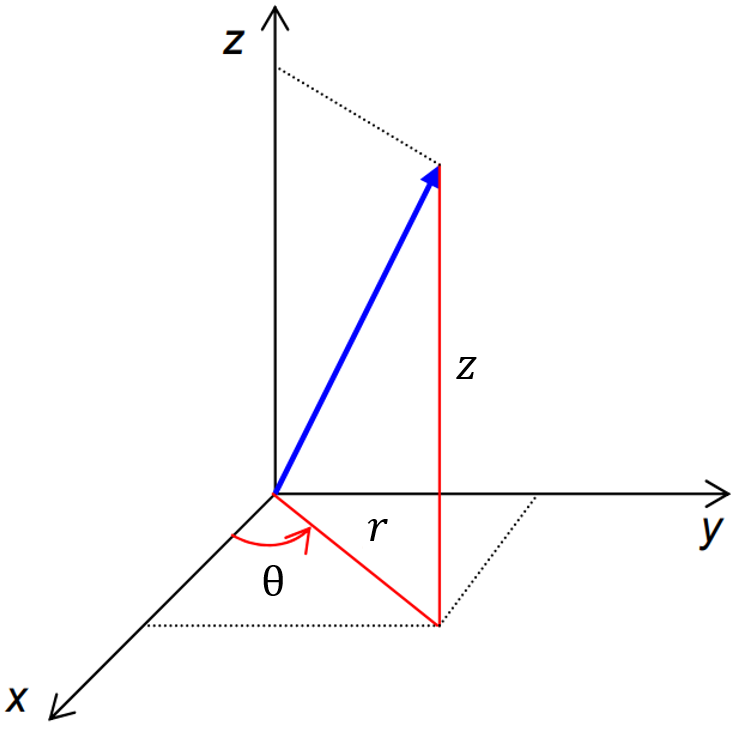
\includegraphics[scale = 0.25]{media/Cylindrical-Coordinates.png}
    \caption{Cartesian and Cylindrical coordinates.}
    \end{center}
\end{figure}
\noindent
The partial derivatives can be evaluated as:
\begin{align*}
\frac{\partial r}{\partial x} &= \frac{x}{r} = \cos(\theta) \qquad \frac{\partial r}{\partial y} = \frac{y}{r} = \sin(\theta) \\
\frac{\partial \theta}{\partial x} &= -\frac{\sin(\theta)}{r} \qquad \quad \; \frac{\partial \theta}{\partial y} = \frac{\cos(\theta)}{r} \\
\end{align*}
\noindent
Applying the chain rule:
\begin{align*}
\frac{\partial \phi}{\partial x} = \frac{\partial \phi}{\partial r} \frac{\partial r}{\partial x} + \frac{\partial \phi}{\partial \theta} \frac{\partial \theta}{\partial x}\\
\frac{\partial \phi}{\partial y} = \frac{\partial \phi}{\partial r} \frac{\partial r}{\partial y} + \frac{\partial \phi}{\partial \theta} \frac{\partial \theta}{\partial y}\\
\end{align*}
\noindent
Therefore, the Laplacian in cylindrical coordinates is

\[ \nabla^2 \;\; = \;\; \frac{\partial^2}{\partial x^2} + \frac{\partial^2}{\partial y^2} + \frac{\partial^2}{\partial z^2} \;\; = \;\; \frac{\partial^2}{\partial r^2} + \frac{1}{r} \frac{\partial}{\partial r} + \frac{1}{r^2} \frac{\partial^2}{\partial \theta^2} + \frac{\partial^2}{\partial z^2} \]
\\ \noindent
and the wave equation can be written as

\[ \frac{1}{c^2} \frac{\partial^2 \phi }{\partial t^2 } = \frac{\partial^2 \phi }{\partial r^2 } + \frac{1}{r} \frac{\partial \phi }{\partial r} + \frac{1}{r^2 } \frac{\partial^2 \phi }{\partial \theta^2 } + \cancel{\frac{\partial^2 \phi }{\partial z^2 }} \quad .\]
\\ \noindent
It is clear that it remains a hyperbolic PDE, but now with a singular point at the origin $r = 0$. The study of surface deformation requires only plane-polar coordinates, so the $\partial^2 \phi / \partial z^2$ term may be neglected. We now seek an analytical solution to the 2-D equation, given well-posed boundary and initial conditions.

\newpage
\subsection{\textbf{Problem Statement}}
\noindent Note: this problem was adapted from Problem Set 9, Exercise 3 of Princeton University Course MAE501: Mathematical Methods of Engineering Analysis I given in Fall semester 2023.
\\ \\
\noindent For a small deformation of any planar circular elastic material, the surface deformation, $\phi$, satisfies the wave equation in plane-polar coordinates

\[ \frac{\partial^2 \phi}{\partial t^2} = c^2 \left[ \frac{1}{r} \frac{\partial}{\partial r} \left(r \frac{\partial \phi}{\partial r}\right) + \frac{1}{r^2} \frac{\partial^2 \phi}{\partial \theta^2} \right]\]
\\
\noindent where the driving force of the wave motion for a material initially at rest can be specified through the boundary and initial conditions. Seeking to model waves on the surface of the fluid generated by the motion of the walls, we choose the following boundary and initial conditions. \\ \\
\noindent Boundary Conditions: \\
$ \phi(r=R, \theta, t) = A \cos(\omega t) \cos (\theta) $ \\
$ \phi(r=0, \theta, t) \rightarrow \textrm{finite} $ \\
$ \phi(r, \theta + 2\pi, t) = \phi(r, \theta, t) $ \\ \\
\noindent Initial Conditions: \\
$ \phi(r, \theta, t=0) = 0 $ \\
$ \partial \phi/ \partial t \, (r, \theta, t=0) = 0 $

\subsection{Method of Solution}
We will solve for $\phi$ for all $t$, $\theta$, and $r$ using the method of separation of variables and eigenfunction expansions. We will also determine the resonance condition for the value of $\omega$. 
\\ \\
\noindent Steps in the solution:
\begin{enumerate}
    \item Use Separation of Variables to de-couple the time component and determine the eigenfunctions for the operator with boundary conditions
    \[ \nabla^2 \psi = \left[ \frac{1}{r} \frac{\partial}{\partial r} \left(r \frac{\partial \psi}{\partial r}\right) + \frac{1}{r^2} \frac{\partial^2 \psi}{\partial \theta^2} \right] = - \lambda \psi \]
    \noindent Boundary Conditions: \\
    $ \psi(r=R, \theta) = 0 $ \\
    $ \psi(r=0, \theta) \rightarrow \textrm{finite} $ \\
    $ \psi(r, \theta + 2\pi) = \psi(r, \theta) $ \\
    \item Determine a function $\tilde{\phi}$, that when subtracted from $\phi$ makes the boundary conditions homogeneous but perhaps introduces inhomogeneities in the initial conditions and the equation itself.
    \item Use the eigenfunctions determined from the separation of variables in the method of eigenfunction expansions and solve for $\phi$.
\end{enumerate} 

\newpage
\subsection{Final Solution}
\noindent These conditions lead to the analytical solution 
$$ \phi(r, \theta, t) = A \left(\frac{r}{R} \right)^2 \cos(\omega t) \cos(\theta) + \tilde{\phi} (r, \theta, t)$$ 

\noindent $\tilde{\phi}$ is composed as follows, where $J_\alpha (\cdot)$ is the Bessel function of the 1st kind and order $\alpha$, $\eta$ is a variable of integration, and $\lambda$ are the eigenfunctions for each of the modes.
$$ \tilde{\phi} (r, \theta, t) = \sum_{m=1}^\infty \Biggl( \frac{1}{c^2 \lambda_{m,n} - \omega^2} \frac{2A}{R^2} \frac{\int_0^1 \left( \omega^2 \eta^2 + 3c^2 \right) \eta J_1\left( \sqrt{\lambda_{1,m}} R \eta \right) d\eta }{{J_2}^2 \left( \sqrt{\lambda_{1,m}} R \right)} \cos(\omega t) \; \dots $$

$$ - \frac{2A}{{J_2}^2 \left( \sqrt{\lambda_{1,m}} R \right)}\Bigg[ \int_0^1 \eta^3 J_1 \left( \sqrt{\lambda_{1,m}} R\eta \right) d\eta \; \dots $$

$$ + \frac{1}{c^2 \lambda_{m,n} - \omega^2} \frac{1}{R^2} \int_0^1 \left(\omega^2 \eta^2 + 3c^2 \right) \eta J_1 \left(\sqrt{\lambda_{1,m}} R \eta \right) d\eta \Bigg] \cos \left(c \sqrt{\lambda_{1,m}} t \right) \Biggl) \cos(\theta) J_1 \left(\sqrt{\lambda_{1,m} } r \right) .$$

\subsection{Full Derivation}
\noindent The method of Separation of Variables can be applied to a partial differential equation (PDE) when the equation is linear and homogeneous, where the boundary conditions are also linear and homogeneous. Thus, considering the homogeneous stationary boundary value problem, using separation of variables, assume $\phi(r, \theta, t) = \psi (r, \theta) \mathcal{T} (t)$ and substituting in the wave equation

\[ \frac{\partial^2 (\psi \mathcal{T})}{\partial t^2} = c^2 \left[ \frac{1}{r} \frac{\partial}{\partial r} \left(r \frac{\partial (\psi \mathcal{T})}{\partial r}\right) + \frac{1}{r^2} \frac{\partial^2 (\psi \mathcal{T})}{\partial \theta^2} \right] \quad \rightarrow \quad \psi \mathcal{T}'' = c^2 \left[ \frac{\mathcal{T}}{r} \frac{\partial}{\partial r} \left(r \frac{\partial \psi}{\partial r}\right) + \frac{\mathcal{T}}{r^2} \frac{\partial^2 \psi}{\partial \theta^2} \right] \quad .\]
\\ \noindent
Dividing by $\psi \mathcal{T} c^2$,

\[ \frac{1}{\psi} \left[ \frac{1}{r} \frac{\partial}{\partial r} \left(r \frac{\partial \psi}{\partial r}\right) + \frac{1}{r^2} \frac{\partial^2 \psi}{\partial \theta^2} \right] = \frac{1}{c^2} \frac{\mathcal{T}''}{\mathcal{T}} = - \lambda \quad ,\]
\\ \noindent
with $\lambda$ a constant that will be shown to correspond to the eigenfunctions for each of the modes. Now using separation of variables again on the spatial component, assume $ \psi (r, \theta) = \mathcal{R}(r) \, \Theta(\theta) $ and again substitute into the $\nabla^2 \psi$ operator

\[ \frac{1}{r} \frac{\partial}{\partial r} \left(r \frac{\partial (\mathcal{R} \Theta)}{\partial r}\right) + \frac{1}{r^2} \frac{\partial^2 (\mathcal{R} \Theta)}{\partial \theta^2} = - \lambda \mathcal{R} \Theta \quad \rightarrow \quad \frac{\Theta}{r} (\mathcal{R}' + r \mathcal{R}'') + \frac{\mathcal{R} \Theta''}{r^2} = - \lambda \mathcal{R} \Theta \quad .\]
\noindent
The PDE can then be rewritten as

\[ \frac{1}{\mathcal{R}} r \frac{d}{dr} \big(r \mathcal{R'} \big) + \lambda r^2 = -\frac{\Theta''}{\Theta}  = \alpha^2 \]
\\ \noindent
with $\alpha^2$ as some constant. First solving the angular component by applying an integrating factor and solving for the roots of the characteristic polynomial $\Theta \sim \exp(\delta \theta) \rightarrow \delta = \pm \alpha i$, then substituting Euler's identity $\exp(i \alpha) = \cos(\alpha) + i \, \sin(\alpha)$. 

\[ \Theta'' = -\alpha^2 \Theta \quad \rightarrow \quad \Theta (\theta) = a \cos(\alpha \theta) + b \sin(\alpha \theta) \quad .\]
\noindent
Applying the condition $\psi(r, \theta + 2\pi) = \psi(r, \theta)$,
\begin{equation*}
    \begin{split}
        a &\cos(\alpha \theta + \alpha 2 \pi) + b \sin(\alpha \theta + \alpha 2 \pi) = a \cos(\alpha \theta) + b \sin(\alpha \theta) \\
        &\rightarrow  \cos(\alpha \theta + \alpha 2 \pi) = \cos(\alpha \theta) \quad \textrm{and} \quad \sin(\alpha \theta + \alpha 2 \pi) = \sin(\alpha \theta) \\
        &\rightarrow \alpha_n = n \in \mathbb{Z}^{\geq 0} \;\; \textrm{an integer}
    \end{split}
\end{equation*}

\noindent
Therefore a solution to the angular problem is

\[\Theta_n (\theta) = a_n \cos(n \theta) + b_n \sin(n \theta) \quad . \]
\newpage
\noindent
Now re-arranging the radial problem (where the substitution $\alpha_n = n$) is made,

\[ \frac{1}{\mathcal{R}} r \frac{d}{dr} \big(r \mathcal{R'} \big) + \lambda r^2 = n^2 \quad \rightarrow \quad r \frac{d}{dr} \big(r \mathcal{R'} \big) + (\lambda r^2 - n^2) \mathcal{R} = 0 \]

\[ r^2 \mathcal{R}'' + r \mathcal{R}' + (\lambda r^2 - n^2) \mathcal{R} = 0 \]
\noindent 
This is the form of a Bessel equation of order $n$ and therefore the solutions to the radial problem are the Bessel functions of order $n$,

\[\mathcal{R}(r) = c J_n (\sqrt{\lambda} r) + d \cancel{Y_n (\sqrt{\lambda} r)} \quad .\]

\noindent
Applying boundary conditions: \\
\noindent $\mathcal{R}(r = 0) \; \textrm{finite} \; \rightarrow \; d = 0$ \\
\noindent $\mathcal{R}(r = R) = 0 \; \rightarrow \; c J_n (\sqrt{\lambda_{n,m}} r) = 0 \; \rightarrow \; \sqrt{\lambda_{n,m}} r = z_{n,m} \; \textrm{for} \; c \neq 0$ \\ \\ \noindent
This gives a relation between the eigenvalues and zeroes of the Bessel function,  where $z_{n,m}$ is the $m$th zero of the $n$th order Bessel function $J_n$ for $m = 1,2,3 \dots$ Therefore the eigenfunctions  are of the form 

\[ \psi_{n,m} (r, \theta) = \mathcal{R}(r) \, \Theta(\theta) = [a_{n,m} \cos(n \theta) + b_{n,m} \sin(n \theta)] J_n (\sqrt{\lambda_{n,m}} r) \]
\\ \noindent
With the modes of $a_{n,m}(t)$ and $b_{n,m}(t)$ to be determined as functions of time. Now considering the original problem, the boundary condition is inhomogeneous, so we must rescale the problem to achieve homogeneous boundary conditions. Let

\[ \tilde{\phi} \equiv \phi - A \left(\frac{r}{R} \right)^2 \cos(\omega t) \cos(\theta) \]
\noindent
Here the $r^2 / R^2$ term is necessary to resolve the singularity from the ODE. Taking the time and spatial derivatives of $\tilde{\phi}$ to rewrite the PDE:

\begin{align*}
\frac{ \partial \phi}{\partial t} &= \frac{ \partial \tilde{\phi}}{\partial t} - A \omega \left(\frac{r}{R} \right)^2 \sin(\omega t) \cos(\theta) \\
\frac{ \partial \phi}{\partial r} &= \frac{ \partial \tilde{\phi}}{\partial r} - 2 A \left(\frac{r}{R^2}\right) \cos(\omega t) \cos(\theta) \\
\frac{ \partial^2 \phi}{\partial t^2} &= \frac{ \partial^2 \tilde{\phi}}{\partial t^2} - A \omega^2 \left(\frac{r}{R} \right)^2 \cos(\omega t) \cos(\theta) \\
\frac{1}{r} \frac{\partial}{\partial r} (r \frac{\partial \phi}{\partial r}) &= \frac{1}{r} \frac{\partial}{\partial r} (r \frac{\partial \tilde{\phi}}{\partial r}) + 4 A \left(\frac{1}{R^2}\right) \cos(\omega t) \cos(\theta) \\
\frac{1}{r^2} \frac{\partial^2 \phi }{\partial \theta^2} &= \frac{1}{r^2} \frac{\partial^2 \tilde{\phi} }{\partial \theta^2} - A \left(\frac{1}{R^2}\right) \cos(\omega t) \cos(\theta)
\end{align*}
\noindent
Now combining to rewrite the solution in terms of the transformed variable $\tilde{\phi}$,

\[ \frac{ \partial^2 \tilde{\phi}}{\partial t^2} - A \omega^2 \left(\frac{r}{R} \right)^2 \cos(\omega t) \cos(\theta) = c^2 \left[ \frac{1}{r} \frac{\partial}{\partial r} (r \frac{\partial \tilde{\phi}}{\partial r}) + \frac{4A}{R^2} \cos(\omega t) \cos(\theta) + \frac{1}{r^2} \frac{\partial^2 \tilde{\phi} }{\partial \theta^2} - \frac{A}{R^2} \cos(\omega t) \cos(\theta) \right]\]
\noindent
which simplifies as

\[ \frac{ \partial^2 \tilde{\phi}}{\partial t^2} - \frac{A}{R^2} \cos(\omega t) \cos(\theta) (\omega^2 r^2 + 3c^2) = c^2 \left[ \frac{1}{r} \frac{\partial}{\partial r} (r \frac{\partial \tilde{\phi}}{\partial r}) + \frac{1}{r^2} \frac{\partial^2 \tilde{\phi} }{\partial \theta^2} \right] \quad .\]
\newpage
\noindent
The initial and boundary conditions are similarly re-scaled.
\\ \\
\noindent Boundary Conditions: \\
$ \tilde{\phi}(r=R, \theta, t) = 0 $ \\
$ \tilde{\phi}(r=0, \theta, t) \rightarrow \textrm{finite} $ \\
$ \tilde{\phi}(r, \theta + 2\pi, t) = \tilde{\phi}(r, \theta, t) $ \\ \\
\noindent Initial Conditions: \\
$ \tilde{\phi}(r, \theta, t=0) = - A \left( \frac{r^2}{R^2} \right) \cos(\theta) $ \\
$ \partial \tilde{\phi}/ \partial t \, (r, \theta, t=0) = 0 $ \\ \\ \noindent
Note that the boundary conditions are now homogeneous, but one of the initial conditions is inhomogeneous. For convenience, define a function

\[ f(r, \theta , t) \equiv A \left( \frac{1}{R^2} \cos(\omega t) \cos(\theta) (\omega^2 r^2 + 3c^2) \right) \quad .\]
\noindent
Solving the new PDE in $\tilde{\phi}$ we expand the inhomogeneity $f(r, \theta , t)$ in the eigenfunctions of the stationary problem

\[ f(r, \theta , t) = \sum^\infty_{n=0} \sum^\infty_{m=0} [c_{n,m}(t) \cos(n \theta) + d_{n,m}(t) \sin(n \theta) ] J_n (\sqrt{\lambda_{n,m}} r) \]
\noindent
Using orthogonality of eigenfunctions we can solve for $c_{n,m}(t)$ and $d_{n,m}(t)$ by calculating the inner product using an appropriate weight function $r$

\[ c_{n,m}(t) = \frac{\langle f(r, \theta, t), J_n (\sqrt{\lambda_{n,m}} r) \cos(n \theta) \rangle_r}{\langle J_n (\sqrt{\lambda_{n,m}} r) \cos(n \theta), J_n (\sqrt{\lambda_{n,m}} r) \cos(n \theta) \rangle_r} = \frac{\int^R_0 \int^{2 \pi}_0 f(r, \theta , t) r J_n (\sqrt{\lambda_{n,m}} r) \cos(n \theta) dr \, d \theta}{\int^R_0 \int^{2 \pi}_0 r {J_n}^2 (\sqrt{\lambda_{n,m}} r) \cos^2(n \theta) dr \, d \theta} \]
\[ d_{n,m}(t) = \frac{\langle f(r, \theta, t), J_n (\sqrt{\lambda_{n,m}} r) \sin(n \theta) \rangle_r}{\langle J_n (\sqrt{\lambda_{n,m}} r) \sin(n \theta), J_n (\sqrt{\lambda_{n,m}} r) \sin(n \theta) \rangle_r} = \frac{\int^R_0 \int^{2 \pi}_0 f(r, \theta , t) r J_n (\sqrt{\lambda_{n,m}} r) \sin(n \theta) dr \, d \theta}{\int^R_0 \int^{2 \pi}_0 r {J_n}^2 (\sqrt{\lambda_{n,m}} r) \sin^2(n \theta) dr \, d \theta} \]
\noindent
We can rewrite 

\begin{multline*}
\int^R_0 \int^{2 \pi}_0 f(r, \theta , t) \, r J_n (\sqrt{\lambda_{n,m}} r) \cos(n \theta) \, dr \, d \theta \;=\\ \frac{A}{R^2} \cos(\omega t) \left[ \int^{2 \pi}_0 \cos(\theta) \cos(n \theta) \, d \theta \int^R_0 (\omega^2 r^2 + 3c^2)  r J_n (\sqrt{\lambda_{n,m}} r) \, d r \right]
\end{multline*}
\noindent
Because $\cos(n \theta)$ are orthogonal functions, only when $n = 1$ is $c_{n,m}$ non-zero.

\[ \int^{2 \pi}_0 \cos(\theta) \cos(n \theta) d \theta = 
\begin{cases}
      \pi & \text{if $n=1$}\\
      0 & \text{if $n \neq 1$}\\
    \end{cases}
\]
\noindent
Thus $c_{n,m}$ simplifies to 

\[ c_{n,m} = 
\begin{cases}
      0 & \text{if $n \neq 1$}\\
      \frac{2A}{R^4} \cos(\omega t) \frac{\int^R_0 (\omega^2 r^2 + 3c^2)  r J_1 (\sqrt{\lambda_{1,m}} r) \, d r}{{J_2}^2 (\sqrt{\lambda_{1,m}} R) } & \text{if $n = 1$}\\
    \end{cases}
\]
\noindent
This also requires the integration property of Bessel functions $\int x^n J_{n-1}(x) dx = x^n J_n(x)$. Similarly, as $f(r, \theta, t)$ is only a function of cosine, 

\[ \int^{2 \pi}_0 \cos(\theta) \sin(n \theta) d \theta = 0 \,\forall \, n \quad \rightarrow \quad d_{n,m} = 0 \; .\]
\newpage
\noindent
Since $\cos(\theta)$ corresponds to $m = 1$ and $\cos(n \theta)$ is orthogonal to $\cos(m \theta)$ for $ n \neq m$, all terms $n \neq 1$ are 0 and the summation over $n$ can be removed.

\[ f(r, \theta , t) = \frac{2A}{R^4} \cos(\omega t) \sum^\infty_{m=1} \frac{\int^R_0 (\omega^2 \zeta^2 + 3c^2)  \zeta J_1 (\sqrt{\lambda_{1,m}} \zeta) d \zeta}{{J_2}^2 (\sqrt{\lambda_{1,m}} R) } \cos(\theta) J_1(\sqrt{\lambda_{n,m}} r)\]
\noindent
Here $\zeta$ is the variable of integration. If we non-dimensionalize the variable in the integral with $R \eta = \zeta$,

\[ f(r, \theta , t) = \frac{2A}{R^2} \cos(\omega t) \sum^\infty_{m=1} \frac{\int^1_0 (\omega^2 \eta^2 + 3c^2)  \eta J_1 (\sqrt{\lambda_{1,m}} R \eta) d \eta}{{J_2}^2 (\sqrt{\lambda_{1,m}} R) } \cos(\theta) J_1(\sqrt{\lambda_{n,m}} r) \quad .\]
\\ \noindent
Similar to the stationary problem, the eigenfunction expansion of $\tilde{\phi}(r, \theta , t)$ is

\[ \tilde{\phi}(r, \theta , t) = \sum^\infty_{n=0} \sum^\infty_{m=1} [a_{n,m}(t) \cos(n \theta) + b_{n,m}(t) \sin(n \theta) ] J_n (\sqrt{\lambda_{n,m}} r) \quad . \]
\\ \noindent
Then we can deduce the following ODE relationships from the PDE:
\begin{align*}
n \neq 1 &: a_{n,m}''(t) = -\lambda_{n,m} \, c^2 \, a_{n,m}(t) \\
n = 1 &: a_{1,m}''(t) - c_{1,m}(t) = -\lambda_{1,m} \, c^2 \, a_{1,m}(t) \\
\forall \, n &: b_{n,m}''(t) = -\lambda_{n,m} \, c^2 \, b_{n,m}(t) \\
\end{align*}
\noindent
Now using the initial conditions for the PDE to get initial conditions for these coefficient ODEs

\[ \tilde{\phi}(r, \theta , t=0) = -A \, \frac{r^2}{R^2} \cos(\theta) \sum^\infty_{n=0} \sum^\infty_{m=1} [a_{n,m}(0) \cos(n \theta) + b_{n,m}(0) \sin(n \theta) ] J_n (\sqrt{\lambda_{n,m}} r) \quad .\]
\noindent
The initial condition does not have a $\sin(\theta)$ term and therefore $b_{n,m}(0) = 0$. To solve for $a_{n,m}(0)$, we use orthogonality of eigenfunctions and take inner products of both sides with $\cos(n \theta) J_n(\sqrt{\lambda_{n,m}} r)$ and using an appropriate weight function $r$

\begin{align*}
a_{n,m}(0) &= \frac{\langle -A \, \frac{r^2}{R^2} \cos(\theta), J_n(\sqrt{\lambda_{n,m}} r) \cos(n \theta) \rangle_r}{\langle J_n(\sqrt{\lambda_{n,m}} r) \cos(n \theta), J_n(\sqrt{\lambda_{n,m}} r) \cos(n \theta) \rangle_r} \\
&= \frac{\int^R_0 \int^{2 \pi}_0 -A (\frac{r}{R})^2 \cos(\theta) r J_n (\sqrt{\lambda_{n,m}} r) \cos(n \theta) \, dr \, d \theta}{\int^R_0 \int^{2 \pi}_0 r {J_n}^2 (\sqrt{\lambda_{n,m}} r) \cos^2(n \theta) \, dr \, d \theta} \\
&= \frac{\int^R_0 -A (\frac{r}{R})^2 r J_n (\sqrt{\lambda_{n,m}} r) \, dr \int^{2 \pi}_0 \cos(\theta) \cos(n \theta) \, d \theta}{\frac{1}{2} \pi R^2 {J_2}^2 (\sqrt{\lambda_{n,m}} R)}
\end{align*}

\begin{align*}
    &= \begin{cases}
    0 & \textrm{if $n \neq 1$} \\
    \frac{-2A}{R^4 J_{n+1}^2 (\sqrt{\lambda_{n,m}} R)} \int^R_0 r^3 J_1 (\sqrt{\lambda_{1,m}} r) \, dr & \textrm{if $n = 1$}
    \end{cases} \\
    &= \begin{cases}
    0 & \textrm{if $n \neq 1$} \\
    \frac{-2A}{{J_2}^2 (\sqrt{\lambda_{n,m}} R)} \int^1_0 \eta^3 J_1 (\sqrt{\lambda_{1,m}} R \eta) \, d \eta & \textrm{if $n = 1$}
    \end{cases}
\end{align*}
\noindent
This also requires the integration property of Bessel functions $\int x^n J_{n-1}(x) dx = x^n J_n(x)$. Applying the second initial condition

\[ \frac{\partial \tilde{\phi}}{\partial t}(r, \theta , t=0) = 0 = \sum^\infty_{n=0} \sum^\infty_{m=1} [a_{n,m}'(0) \cos(n \theta) + b_{n,m}'(0) \sin(n \theta) ] J_n (\sqrt{\lambda_{n,m}} r) \]
\\ \noindent
implies that $a_{n,m}'(0) = 0$ and $b_{n,m}'(0) = 0$. Now solving the ODEs for $a_{n,m}$ and $b_{n,m}$. First for the case $n \neq 1$, by applying an integrating factor and solving for the roots of the characteristic polynomial $a \sim \exp(\delta t) \rightarrow \delta = \pm c \sqrt{\lambda_{n,m}} i$, then substituting Euler's identity $\exp(i c \sqrt{\lambda_{n,m}} t) = \cos(c \sqrt{\lambda_{n,m}} t) + i \, \sin(c \sqrt{\lambda_{n,m}} t)$. We use the initial conditions to solve for the constants $\kappa_1$, $\kappa_2$

\[ a_{n,m}(t) = \kappa_1 \cos(c \sqrt{\lambda_{n,m}} t) + \kappa_2 \sin(c \sqrt{\lambda_{n,m}} t) \quad \rightarrow \quad \kappa_1 = 0, \; \kappa_2 = 0 \quad \rightarrow \quad a_{n,m}(t) = 0\]
\\ \noindent
Similarly for all $n$, $b_{n,m}(t) = 0$. For the case $n = 1$:

\[ a_{n,m}''(t) = \frac{2A}{R^2} \cos(\omega t) \, \frac{\int_0^1 \left( \omega^2 \eta^2 + 3c^2 \right) \eta J_1\left( \sqrt{\lambda_{1,m}} R \eta \right) d\eta}{{J_2}^2 \left( \sqrt{\lambda_{1,m}} R \right)} = -c^2 \lambda_{n,m} a_{1,m} \]
\noindent
The homogeneous solution to this ODE is of the form (again using an integrating factor approach)

\[ a_{n,m}^{\textrm{hom}}(t) = \kappa_3 \cos(c \sqrt{\lambda_{n,m}} t) + \kappa_4 \sin(c \sqrt{\lambda_{n,m}} t) \]
\noindent
and by inspection we find a particular solution

\[ a_{n,m}^{\textrm{part}}(t) = \kappa_5 \cos(\omega t) \quad .\]
\noindent
Solving for $k_5$ yields

\[ \kappa_5 = \frac{1}{c^2 \lambda_{n,m} - \omega^2} \frac{2A}{R^2} \frac{\int_0^1 \left( \omega^2 \eta^2 + 3c^2 \right) \eta J_1\left( \sqrt{\lambda_{1,m}} R \eta \right) d\eta}{{J_2}^2 \left( \sqrt{\lambda_{1,m}} R \right)} \quad .\]
\noindent
The general solution for the coefficients is thus

\[ a_{1,m}(t) = \kappa_3 \cos(c \sqrt{\lambda_{n,m}} t) + \kappa_4 \sin(c \sqrt{\lambda_{n,m}} t) + \frac{1}{c^2 \lambda_{n,m} - \omega^2} \frac{2A}{R^2} \frac{\int_0^1 \left( \omega^2 \eta^2 + 3c^2 \right) \eta J_1\left( \sqrt{\lambda_{1,m}} R \eta \right) d\eta}{{J_2}^2 \left( \sqrt{\lambda_{1,m}} R \right)} \cos(\omega t) \; .\]
\noindent
From the initial conditions we find that $\kappa_4 = 0$ and

\[ \kappa_3 = \frac{-2A}{{J_2}^2 \left( \sqrt{\lambda_{1,m}} R \right)} \int_0^1 \eta^3 J_1 \left( \sqrt{\lambda_{1,m}} R \eta \right) d \eta - \frac{1}{c^2 \lambda_{m,n} - \omega^2} \frac{2A}{R^2} \frac{\int_0^1 \left( \omega^2 \eta^2 + 3c^2 \right) \eta J_1\left( \sqrt{\lambda_{1,m}} R \eta \right) d\eta }{{J_2}^2 \left( \sqrt{\lambda_{1,m}} R \right)}\]
\noindent
\textbf{Substituting to write the closed form solution for $\tilde{\phi}$}

$$ \tilde{\phi} (r, \theta, t) = \sum_{m=1}^\infty \Biggl( \frac{1}{c^2 \lambda_{m,n} - \omega^2} \frac{2A}{R^2} \frac{\int_0^1 \left( \omega^2 \eta^2 + 3c^2 \right) \eta J_1\left( \sqrt{\lambda_{1,m}} R \eta \right) d\eta }{{J_2}^2 \left( \sqrt{\lambda_{1,m}} R \right)} \cos(\omega t) \; \dots $$

$$ - \frac{2A}{{J_2}^2 \left( \sqrt{\lambda_{1,m}} R \right)}\Bigg[ \int_0^1 \eta^3 J_1 \left( \sqrt{\lambda_{1,m}} R\eta \right) d\eta \; \dots $$

$$ + \frac{1}{c^2 \lambda_{m,n} - \omega^2} \frac{1}{R^2} \int_0^1 \left(\omega^2 \eta^2 + 3c^2 \right) \eta J_1 \left(\sqrt{\lambda_{1,m}} R \eta \right) d\eta \Bigg] \cos \left(c \sqrt{\lambda_{1,m}} t \right) \Biggl) \cos(\theta) J_1 \left(\sqrt{\lambda_{1,m} } r \right) .$$
\noindent
\textbf{and the solution in the original variable}
$$ \phi(r, \theta, t) = A \left(\frac{r}{R} \right)^2 \cos(\omega t) \cos(\theta) + \tilde{\phi} (r, \theta, t) \quad .$$ 

\noindent By inspection of $\tilde{\phi}(r, \theta, t)$, the coefficient in the summation goes to infinity and ``blows up'' as the denominator $c^2 {\lambda_n}^2 - \omega^2 \rightarrow 0$, thus a resonance condition exists when $c^2 {\lambda_n}^2 = \omega^2$. $c \lambda_n$ can be interpreted as an eigenfrequency which, when excited, results in resonance. 

\end{document}